\chapter{Generar Percusión por Ordenador}
\label{cap:generacionPercusion}

La percusión\footnote{\url{https://rayrojodrums.com/es/que-son-las-percusiones/}} es una parte fundamental de una canción que aporta ritmo y soporte al resto del arreglo musical. Para la generación de percusión hemos barajado dos opciones, la generación usando \cite{MagentaStudio}(más info en la Sección \ref{sec:magenta}) y la implementación de nuestro propio generador. La opción por la que nos hemos decantado finalmente es la de la generación propia, explicada en la Sección \ref{subsec:generacion-percusion-propia}.


\section{Generación de percusión}
\label{sec:generacion-percusion}

    \subsection{Generación de percusión con Magenta}
    \label{subsec:generacion-percusion-magenta}
    \textit{Drumify} es un programa sencillo dentro de la suite de aplicaciones de Magenta. Su uso es simple pero eficaz: se carga un archivo MIDI (Sección \ref{subsec:que-es-midi}) de una canción, ya sea con acordes o sólo melodía, y devuelve un archivo MIDI con un arreglo batería que funciona para la canción proporcionada. 
    
    Este flujo de trabajo se puede completar usando otra herramienta que nos da Magenta, que en la versión de escritorio llaman \textit{Groove}.
    El \textit{groove} en una canción, en este caso aplicado a la parte de la percusión, es algo así como la sensación de movimiento que genera la canción al escucharla\footnote{\url{https://es.wikipedia.org/wiki/Groove_(musica)}}.
    
    La aplicación \textit{Groove} de Magenta recibe un archivo MIDI, esta vez de percusión, y humananiza las notas, poniendo más velocidad en las notas que suenan en los golpes fuertes del compás, que generalmente serán el bombo y muchas veces la caja, mientras que otros instrumentos como los platillos tendrán menos velocidad. También varía ligeramente la posición de las notas, de forma que no quedan colocadas en el instante de tiempo exacto marcado por el compás, algo que hace que la percusión (y todos los instrumentos en general) suenen bastante robóticos.

    \subsection{Generación de percusión propia}
    \label{subsec:generacion-percusion-propia}
    Una vez vistas las herramientas que nos brinda Magenta para la generación de MIDIs de percusión, llegamos a la conclusión de que era algo que, si bien funcionaba, era demasiado genérico para lo que buscábamos. Por esta razón, no usaremos Magenta en la herramienta.
    
    Hemos implementado nuestro propio generador de percusión, que nos permite trabajar mejor en los estilos que buscábamos, que se presentarán en la Sección \ref{subsubsec:estilos-percusion}. Este generador crea tres archivos MIDI de un compás 4/4 de duración del estilo especificado. A continuación, se especifica su funcionamiento.

    \subsection{¿Cómo enfocamos la percusión?}

    %TODO: working example
    Con el fin de poder programar algún tipo de generador de ritmos de batería, vamos a tratar de simplificar al máximo la forma de crear partes de percusión para una canción.

    El enfoque que vamos a darle es similar al que se explica en el vídeo de YouTube del canal "8-bit Music Theory", (\cite{DrumPartsForNoDrummers})

    Separamos las baterías en tres partes principales:

    \begin{itemize}
        \item \textbf{\textit{Beat}}: Suelen ser notas en los golpes fuertes. Es la parte fundamental del ritmo. Generalmente suele ser el bombo el encargado de esta función.
        \item \textbf{\textit{Engine}}: Son golpes que contrastan con el \textit{beat}. Añaden movimiento al ritmo. Si en el \textit{beat} tenemos un bombo en el \textit{engine} podríamos tener una caja. Pueden ir en los golpes fuertes o en los débiles.
        \item \textbf{\textit{Constant}}: No destaca especialmente pero añade consistencia al ritmo. Esta función suelen desempeñarla los platillos. Suelen ir en los golpes débiles.
    \end{itemize}

    Juntando estas tres partes obtenemos un ritmo de batería base que podemos mantener durante una parte o la totalidad de la canción. Podemos ver un ejemplo de este ritmo en la Figura \ref{fig:ritmo-basico-percusion}, donde la línea de abajo representa el \textit{beat}, en este caso un bombo, la de arriba representa la \textit{constant}, en este caso platillos, y la línea central representa el \textit{engine}, en este caso un golpe de caja.

     \begin{figure}[h]
        \centering
        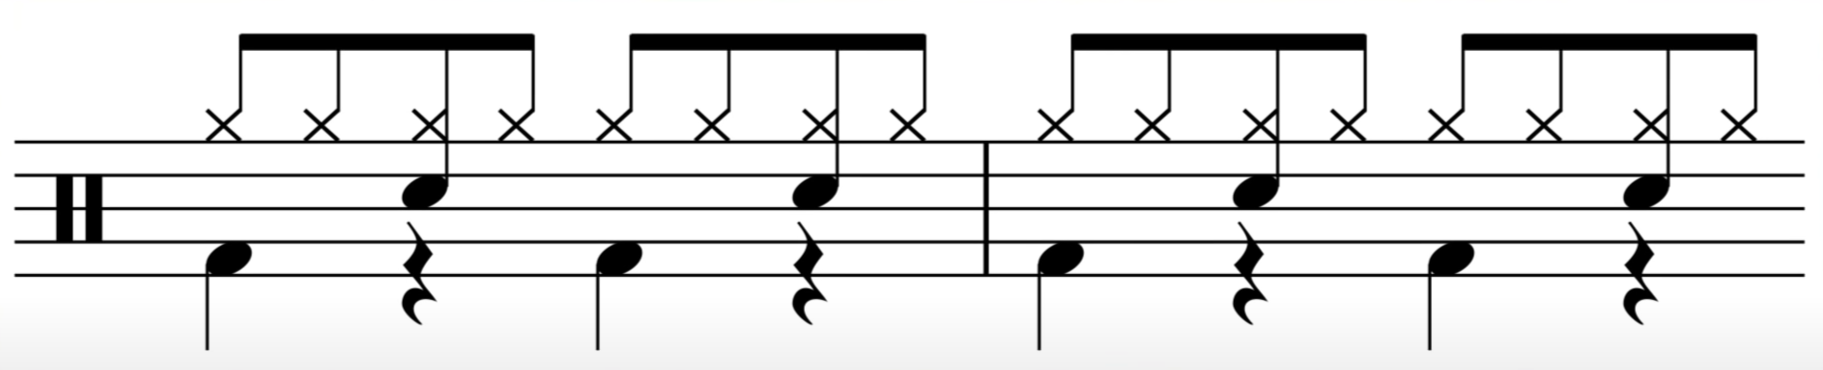
\includegraphics[width = 0.45\textwidth]{Imagenes/Bitmap/BateriaBasico.png}
        \caption{Ritmo básico de percusión.}
        \label{fig:ritmo-basico-percusion}
    \end{figure}

    %TODO: referenciar esta imagen
    \begin{figure}[h]
        \centering
        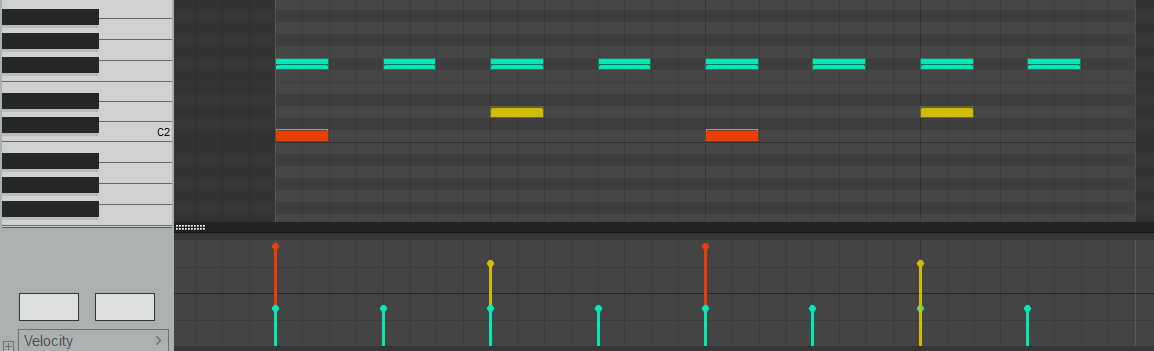
\includegraphics[width = 0.5\textwidth]{Imagenes/Bitmap/PatronPercusionOriginal.png}
        \caption{Ritmo básico de percusión en el rodillo de piano.}
        \label{fig:PatronPercusionOriginal}
    \end{figure}

    %TODO: referenciar esta imagen
    \begin{figure}[h]
        \centering
        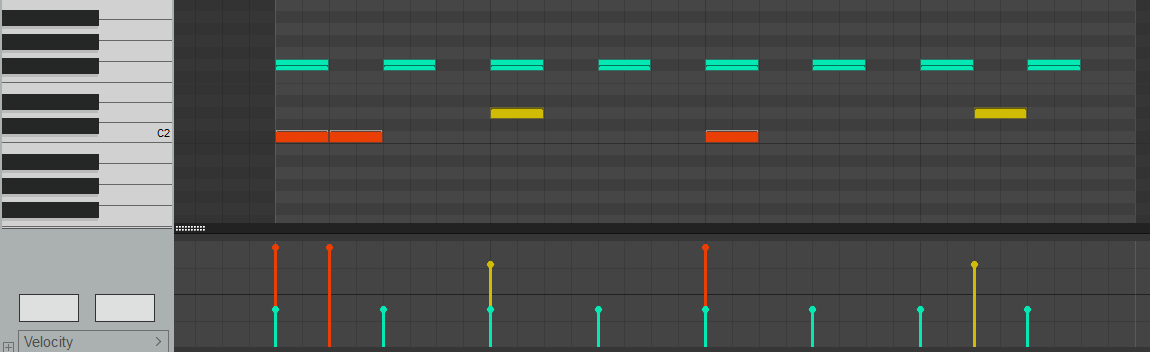
\includegraphics[width = 0.5\textwidth]{Imagenes/Bitmap/PatronPercusionBasico.png}
        \caption{Ejemplo de un patrón de percusión resultante.}
        \label{fig:PatronPercusionBasico}
    \end{figure}

    
    Una vez tenemos el ritmo base, podemos añadir algunos adornos. Algunos ejemplos de adornos podrían los \textit{drum fills} o las intros.

    \subsection{\textit{Drum Fills}}
    \label{subsubsec:generacion-drum-fills}

    Un \textit{drum fill} es un pequeño motivo musical que sirve para añadir variedad a un ritmo de batería y para hacer transiciones entre secciones de un arreglo musical\footnote{\url{https://es.wikipedia.org/wiki/Fill_(musica)}}. A veces los \textit{drum fills} pueden aparecer indicados en las partituras de los bateristas, pero en otras ocasiones sólo viene indicado dónde tocar un \textit{fill} y es el propio baterista el que improvisa un \textit{drum fill}.
    
    La primera idea para lograr tener \textit{drum fills} fue la de implementarlos como el resto de las partes de percusión. Esta idea fue descartada debido a que los \textit{drum fills} usan más elementos de la batería y son más creativos que los ritmos que hemos visto en el punto anterior.

    Por tanto, para obtener \textit{drum fills}, cargamos en REAPER (Sección \ref{sec:reaper}) un archivo MIDI (Sección \ref{subsec:que-es-midi}) con algunas notas de percusión marcadas. A continuación, añadimos a la pista el plugin arpegiador \textit{BlueArp} (Sección \ref{subsubsec:bluearp}) para que arpegie las notas de percusión del ítem MIDI cargado. Por último añadimos un plugin humanizador (Sección \ref{subsubsec:humanizador}) que además de variar la velocidad y \textit{timing} de las notas, varía la nota que se interpreta. Esto lo que hace en un instrumento de batería es cambiar que elemento de la batería se toca. Lo que obtenemos como resultado es una secuencia de golpes de batería generadas de forma aleatoria que al combinar con el ritmo base da como resultado un \textit{drum fill}.

    %TODO: referenciar esta imagen
    \begin{figure}[h]
        \centering
        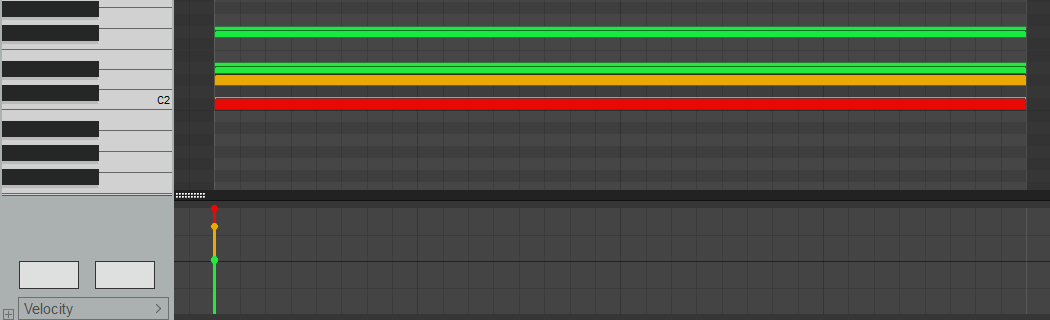
\includegraphics[width = 0.5\textwidth]{Imagenes/Bitmap/FillTemplate.png}
        \caption{Ítem MIDI auxiliar usado para generar \textit{drum fills}}
        \label{fig:FillTemplate}
    \end{figure}
    
    %TODO: referenciar esta imagen
    \begin{figure}[h]
        \centering
        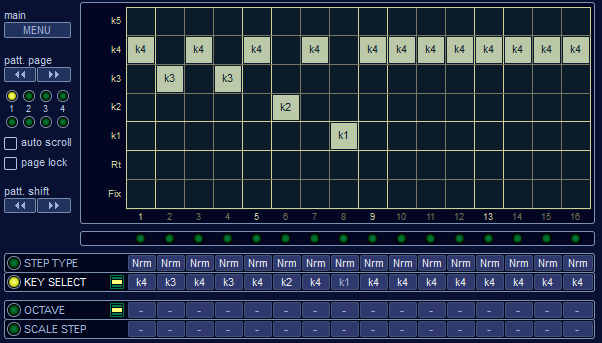
\includegraphics[width = 0.3\textwidth]{Imagenes/Bitmap/FillArp.png}
        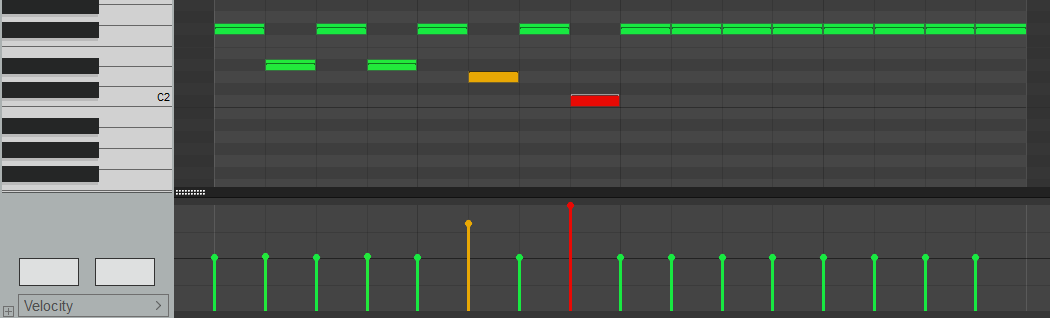
\includegraphics[width = 0.5\textwidth]{Imagenes/Bitmap/FillResult.png}
        \caption{Arpegiador y resultado final de un \textit{drum fill}}
        \label{fig:FillResult}
    \end{figure}

    Además, si esta secuencia que hemos generado suena sin el ritmo base, cumple la función de una intro de batería, que da pie a que entre el ritmo al comienzo del siguiente compás.

    Los \textit{drum fills} los colocaremos cada  4 compases, siendo cada 8 algo más largos, al igual que cuanto más avanzado se encuentren en la canción.


    
    
    \subsubsection{Estilos}
    \label{subsubsec:estilos-percusion}
    Todos los patrones que se generen serán variaciones de un patrón básico. Por ejemplo, en la Figura \ref{fig:Partituras-percusión} podemos ver un patrón básico de batería como el que vimos anteriormente y a su derecha un patrón de jazz. Si nos fijamos, podemos observar que el \textit{beat} y el \textit{engine} son similares, cambiando los golpes de percusión con los que se tocan dichas partes (platillos en ambos casos). 

    \begin{figure}[h]
        \centering
        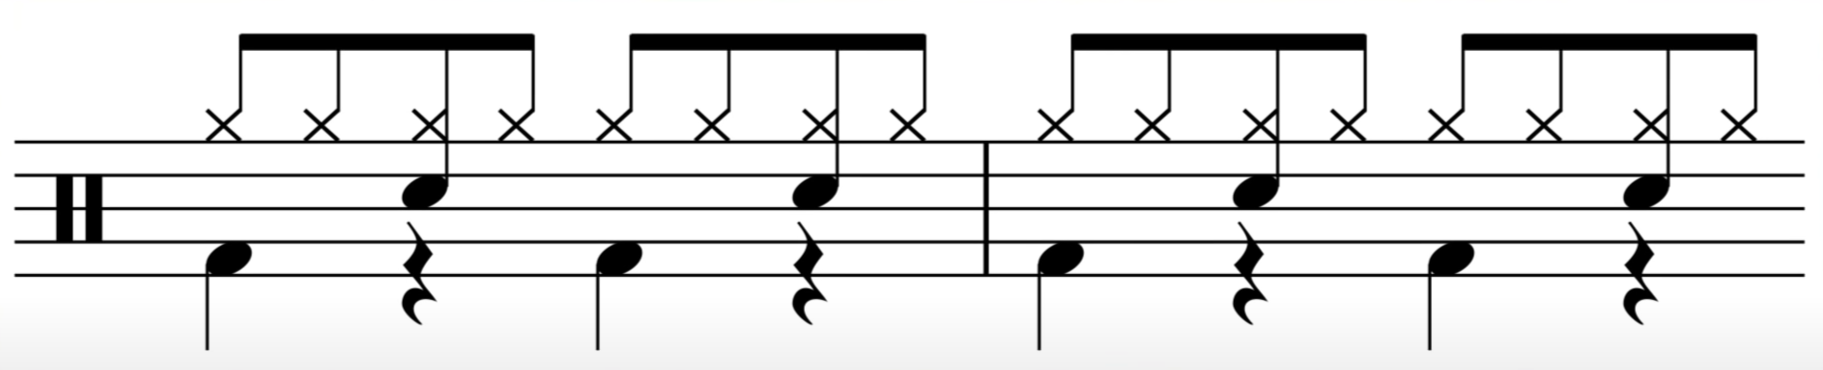
\includegraphics[width = 0.45\textwidth]{Imagenes/Bitmap/BateriaBasico.png}
        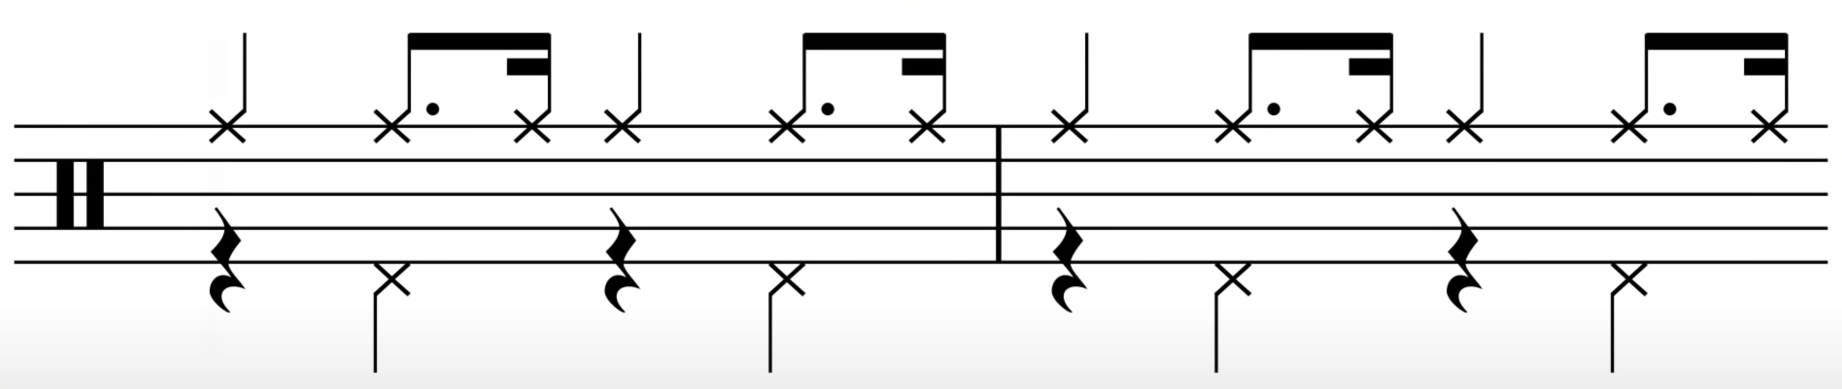
\includegraphics[width = 0.45\textwidth]{Imagenes/Bitmap/BateriaJazz.png}
        \caption{A la izquierda ritmo estándar básico de percusión, a la derecha ritmo estándar de jazz.}
        \label{fig:Partituras-percusión}
    \end{figure}
    
    Lo patrones básicos son los propios de varios géneros musicales. Con estos patrones tratamos de cubrir la mayor parte de ritmos posibles. Son los siguientes:
    
    \begin{itemize}
        \item \textbf{Estilo básico}: Ritmo más básico de bombo y caja con platillos como \textit{constant}.
        \item \textbf{Palmas}: Ritmo de palmas con varias voces simultaneas
        \item \textbf{Maracas}: Ritmo con una maraca como \textit{constant} con un bombo ocasional.
        \item \textbf{Jazz}: Platillos como \textit{beat} y haciendo un ritmo contrastante como \textit{constant} y un platillo de pedal haciendo el engine.
        \item \textbf{Disco}: Bombo a negras con caja y platillos.
        \item \textbf{Metal}: Platillos haciendo el \textit{beat} y doble bombo como \textit{constant}
        \item \textbf{Latin}: Bombo, caja y platillos haciendo ritmos que contrastan entre sí.
        \item \textbf{Rock}: Caja haciendo el \textit{beat} y bombo la \textit{constant}
        \item \textbf{Dembow}: Bombo y caja en el que cada segunda caja se retrasa ligeramente.
    \end{itemize}
    

    
    \subsubsection{Generación de patrones}
    \label{subsubsec:generacion-patrones}
    Para simplificar la representación interna a la hora de generar variedad entre patrones, generamos de forma independiente las partes del beat, del engine y del constant.
    
    Se parte de un patrón de batería básico, como los de la Figura \ref{fig:Partituras-percusión}. De manera aleatoria se decide saltarse algunas notas, adelantarlas, tocar dos veces en lugar de una, etc. De esta forma obtenemos un patrón de batería derivado de uno de los patrones básicos.

    Codificamos cada parte (\textit{beat}, \textit{engine} y \textit{constant}) como arrays de 16 unidades de tamaño y asignamos a cada elemento del array la duración de una semicorchea, por lo que el patrón resultante es un compás 4/4 dividido como máximo en semicorcheas. Variando ligeramente este patrón, crearemos otros dos que serán muy similares entre ellos y al original.

    \subsubsection{Combinación de patrones}
    \label{subsubsec:combinacion-patrones}
        
    Como se ha explicado en el punto anterior, hemos generado tres patrones distintos de un mismo estilo que además funcionan bien juntos. Llamaremos a estos patrones A, B y C.
    
    Es común en los arreglos de percusión combinar estos patrones de cierta manera para añadir variedad al ritmo básico. Por ejemplo, podemos encontrarnos una secuencia bastante común ABAC o una secuencia AABB, que no sería más que tocar de una en una en secuencia los patrones correspondientes, volviendo a empezar al llegar al final de la secuencia.
    
    Estas secuencias las generamos de manera aleatoria una vez, por lo que para cada canción generada saldrá una secuencia distinta pero a lo largo de una canción la batería mantiene esa secuencia continuamente.
    
    Dependiendo de la temática escogida para la canción, se cargarán unos estilos de batería u otros, generalmente tres estilos distintos que van cambiando a lo largo de la canción de manera aleatoria.

    
    %TODO: referenciar esta imagen
    \begin{figure}[h]
        \centering
        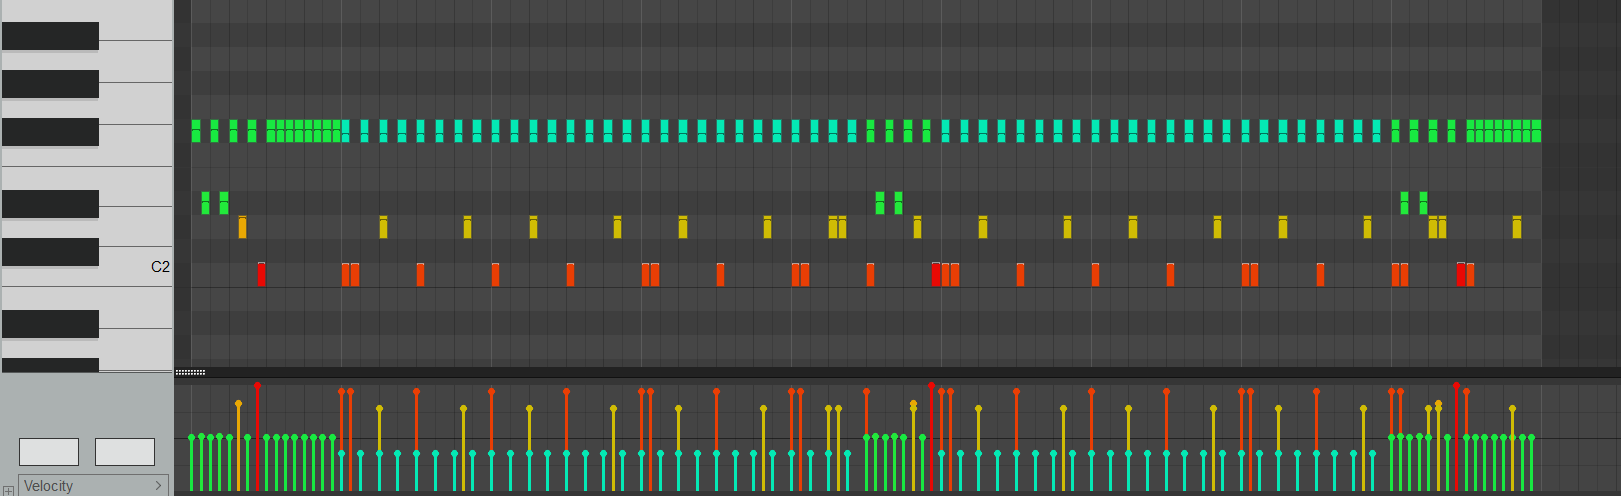
\includegraphics[width = 0.9\textwidth]{Imagenes/Bitmap/RitmoCompleto.png}
        \caption{Ritmo resultante completo}
        \label{fig:RitmoCompleto}
    \end{figure}
    
    \subsubsection{Percusión en MIDI}
    \label{subsubsec:percusion-midi}

A la hora de interpretar un archivo MIDI (Sección \ref{subsec:que-es-midi}) de percusión, la mayoría de instrumentos virtuales mapean las notas de la misma forma. Por ejemplo el bombo es la nota MIDI 36 y la caja la nota MIDI 38 (Do3 y Re3 respectivamente).

La velocidad de las notas MIDI en los instrumentos de percusión indican con cuanta fuerza se realiza el golpe. En algunos instrumentos virtuales la velocidad de la nota se ignora, en otros se reproduce el sonido correspondiente con más o menos volumen y en otros instrumentos hay muestras específicas grabadas para distintas velocidades de la nota. Asimismo, es común que en los instrumentos virtuales de percusión haya varias muestras para una misma nota y una misma velocidad, con el fin de que no suene siempre el mismo golpe exacto y el ritmo resultante suene más realista.